
\begin{figure}[h!]
    \centering
    \caption{Estimates of the effect of the MW on rents, county by month data}
    \label{fig:dynamic_county_month}

	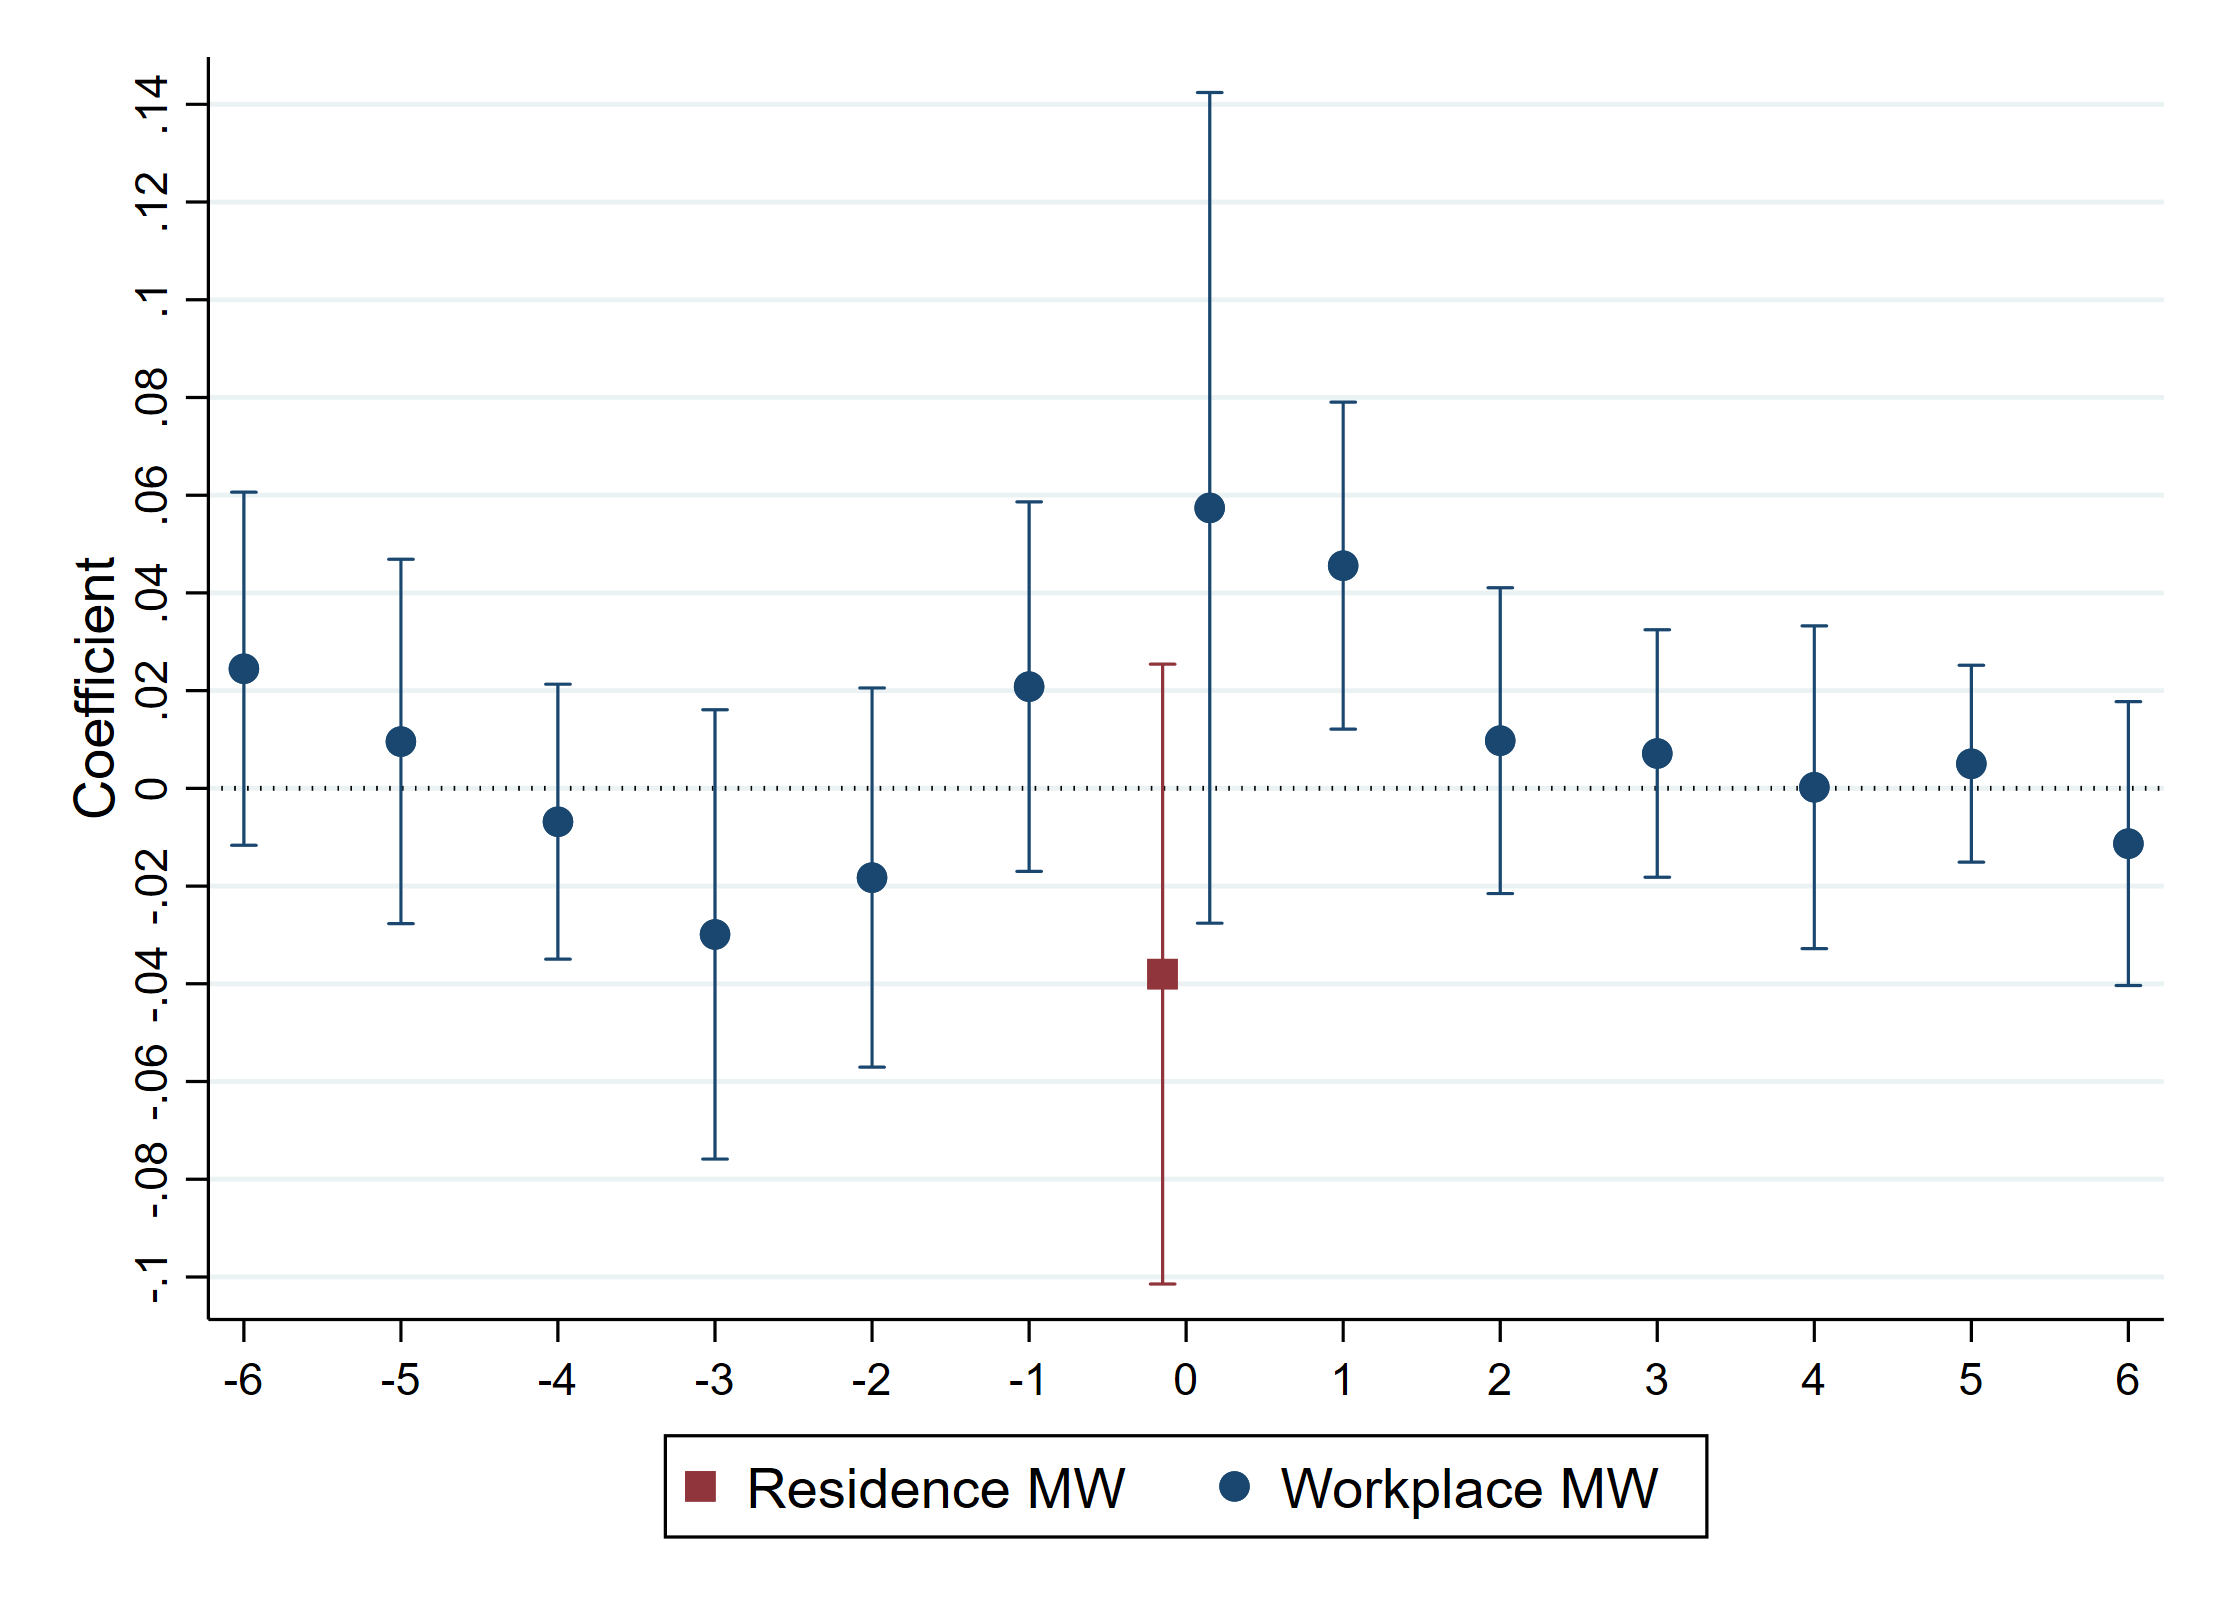
\includegraphics[width = 0.75\textwidth]{fd_geos_times/output/fd_both_mw_wkp_only_dynamic.png}

    \begin{minipage}{.95\textwidth} \footnotesize
        \vspace{3mm}
        Notes:
        Data are from the a county by month panel described in Section 
        \ref{sec:data_final_panel}.
        We plot coefficients from regressions of the log of rents per
        square foot on the residence and workplace MW measures, including 
        six leads and lags of the workplace MW measure.
        All regressions are estimated in first differences and include 
        time-period fixed effects and economic controls that vary at the 
        county and month levels.
        The measure of rents per square foot correspond to the Single Family, 
        Condominium and Cooperative houses from Zillow.
        The residence MW is defined as the log statutory MW at the County.
        The workplace MW is defined as the log statutory MW where the average 
        resident of the county works, constructed using LODES 
        origin-destination data.
        Economic controls from the QCEW include the change of the following 
        variables: the log of the average wage, the log of employment, and the 
        log of the establishment count for the sectors ``Information,'' 
        ``Financial activities,'' and ``Professional and business services.''
        95\% pointwise confidence intervals are obtained from standard errors 
        clustered at the state level.
    \end{minipage}
\end{figure}
